\chapter{Лекция 2 — 17 февраля 2025}

\section{Функции}

Программа на Lisp представляет собой вызов функции на верхнем уровне.
Синтаксически программа оформляется в виде S-выражения. 

При создании программы используются стандартные функции Lisp и функции пользователя. 
Стандартные функции Lisp носят частичный характер,
то есть работают не всегда корректно с поданными аргументами.
Функции всюду определимы в Lisp, то есть если функция приняла 
аргументы, то что-то должна вернуть в любом случае.

\begin{listbox}{\noindent \begin{listboxtitle}{}2\end{listboxtitle} 
    \raisebox{6pt}{Способы определения функций:}}
\begin{enumerate}
	\item lambda-нотация (функция без имени);
	\item с использованием макро определения(спец функции) DEFUN.
\end{enumerate}
\end{listbox}

\begin{figure}[H]
    \begin{listingbox}{}
        \lstinputlisting[language=Lisp]{lists/lambda-defun.lisp}

        \textlambda-выражение  = (lambda \textlambda-список форма).

        Вызов: (\textlambda-выражение форма1 ... формаN)
    \end{listingbox}
    \caption{Примеры вызова defun и lambda функций}
    \label{lst:lambda-defun-example}
\end{figure}

Вычисление функций и выполнение программ осуществляет интерпретатор eval.
Вычисление функций без имени может быть выполнено с помощью функционала apply или funcall.
Вместо циклов и операторов используются рекурсивные функции.

\section{Классификация функций}

\begin{listbox}{\noindent \begin{listboxtitle}{}6\end{listboxtitle}}
\begin{enumerate}
	\item чистые -- (так, как принято в математике, вычисляются все аргументы);
	\item специальные(формы) -- переменное кол-во аргументов или они обрабатываются 
    по-разному, могут вычисляться не все (cond, if, and, or, quote, eval, lambda).
	\item псевдофункции -- создают спецэффекты (например -- вывод на экран);
	\item с вариантыми значениями;
	\item высших порядков(функционалы) -- в качестве аргумента используют другие 
    функции или возвращают функцию в качестве результата(apply, funcall);
    \item базисные функции.
\end{enumerate}
\end{listbox}

\section{Классификация базисных функций}

\begin{listbox}{\noindent \begin{listboxtitle}{}3\end{listboxtitle}}
\begin{enumerate}
    \item Селекторы -- car, cdr;
    \item Функции-конструкторы:
    \begin{itemize}[label=—]
        \item cons -- создает списковую ячейку и расставляет указатели, передается 
        2 S-выражения;
        \item list -- (не базисная форма) создает столько списковых ячеек, 
        сколько аргументов, менее эффективная;
    \end{itemize}
    \item Предикаты -- логические функции:
    \begin{itemize}[label=—]
        \item null -- пустая ли структура;
        \item atom -- является ли атомом;
        \item consp -- является ли структура точечной парой;
        \item listp -- список или нет(более качественная проверка относительно consp);
        \item eq -- проверяет, ссылаются ли два объекта на одно и то же место в памяти. Подходит для символов, точечных пар.
        \item eql -- сравнивает атомы и числа одного типа (= применима только к числам, любого типа), не сравнивает списки;
        \item equal -- eql + списки, но не сравнивает числа разных типов (2 и 2.0);
        \item equalp -- сравнивает всё.
    \end{itemize}
\end{enumerate}
\end{listbox}

\section{Символ апостроф}

Апостроф эквивалентен вызову функции quote. Она позволяет заблокировать 
вычисление своего единственного аргумента:

\begin{figure}[H]
    \begin{listingbox}{}
        '(A B C) == (quote (A B C))
    \end{listingbox}
    \caption{Синтаксис апострофа}
\end{figure}

\section{eval}

Функция EVAL - это функция, которая может вычислить любое правильно составленное 
выражение языка LISP.

\begin{figure}[H]
    \begin{listingbox}{}
        \lstinputlisting[language=Lisp]{lists/eval.lisp}
    \end{listingbox}
    \caption{Пример работы функции eval}
    \label{lst:eval-example}
\end{figure}

\begin{figure}[H]
    \begin{imagebox}
        \centering
        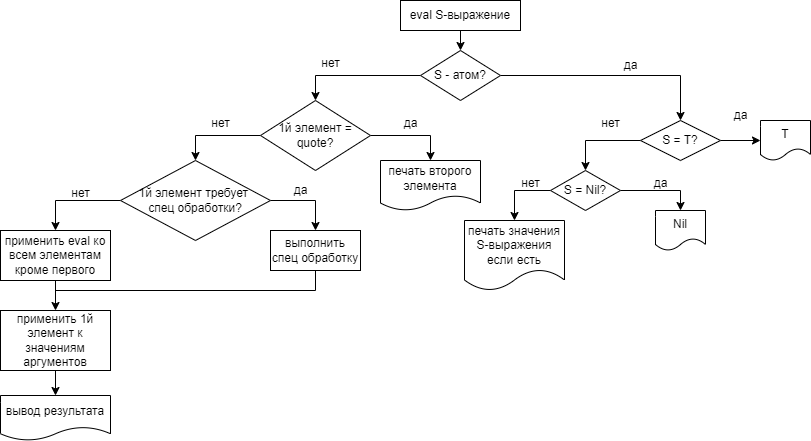
\includegraphics[width=0.9\textwidth]{img/eval.drawio.png}
        \label{fig:eval-sheme}
    \end{imagebox}
    \caption{Схема работы функции eval}
\end{figure}